Sensor LiDAR berperan sebagai sumber utama informasi geometris lingkungan dalam sistem navigasi yang diusulkan. Data hasil pemindaian digunakan untuk mendeteksi obstacle di sekitar robot, mengukur jarak terhadap obstacle terdekat, serta mengestimasi tingkat keterlaluan (\textit{traversability}) area di depan robot. Informasi tersebut selanjutnya digunakan pada proses fusi sensor dan pengambilan keputusan navigasi.

Berbeda dengan kamera termal yang menghasilkan representasi lingkungan dalam bentuk citra, LiDAR menghasilkan data jarak yang bersifat langsung dan memiliki ketelitian spasial yang tinggi. Oleh karena itu, sensor ini tetap menjadi komponen utama dalam proses perencanaan lintasan dan penghindaran obstacle pada penelitian ini (\cite{Fagundes2024,Liu2024}).

\subsection{Akuisisi Data LiDAR}

Sensor LiDAR menghasilkan data pindaian dalam format \texttt{sensor\_msgs/LaserScan} y\-ang dipublikasikan melalui topik \texttt{/scan}. Data tersebut terdiri atas sekumpulan pasangan sudut dan jarak yang merepresentasikan obstacle pertama yang terdeteksi pada setiap arah pengamatan.

Pada penelitian ini, sensor LiDAR memiliki cakupan pemindaian horizontal sebesar 360$^\circ$ dengan frekuensi pembaruan 40 Hz. Setiap siklus pemindaian menghasilkan 720 sampel jarak yang mencakup seluruh area di sekitar robot. Data tersebut digunakan secara simultan oleh ROS Navigation Stack dan APFPlanner untuk membangun representasi lingkungan lokal.

\subsection{Keterbatasan Blind-Spot Vertikal LiDAR}

Meskipun mampu memberikan informasi jarak secara akurat, LiDAR dua dimensi memiliki keterbatasan inheren karena hanya melakukan pemindaian pada satu bidang horizontal dengan ketinggian tetap terhadap lantai. Akibatnya, obstacle yang seluruh profilnya berada di bawah bidang pindai tidak akan menghasilkan pantulan laser dan tidak dapat dideteksi oleh sensor (\cite{Kibii2022,Fagundes2024}).

Secara konseptual, suatu obstacle hanya dapat dideteksi apabila sebagian profil objek memotong bidang pindai LiDAR. Jika seluruh bagian obstacle berada di bawah bidang tersebut, maka obstacle akan berada pada area \textit{blind-spot}. Kondisi ini umum dijumpai pada robot bergerak yang menggunakan LiDAR dua dimensi untuk navigasi dalam ruangan, khususnya ketika berhadapan dengan obstacle berprofil rendah seperti hewan peliharaan, benda kecil di lantai, atau objek yang memiliki tinggi lebih rendah dibandingkan posisi sensor.

Pada penelitian ini, kondisi tersebut direpresentasikan melalui obstacle kucing (\texttt{obstac\-le\_cat}) yang memiliki tinggi lebih rendah dibandingkan bidang pindai LiDAR. Akibatnya, obstacle tersebut tidak dapat terdeteksi oleh sensor laser meskipun berada tepat pada jalur pergerakan robot. Keterbatasan inilah yang menjadi dasar penggunaan kamera termal sebagai sensor pelengkap untuk meningkatkan kemampuan persepsi lingkungan.

\begin{figure}[H]
\centering
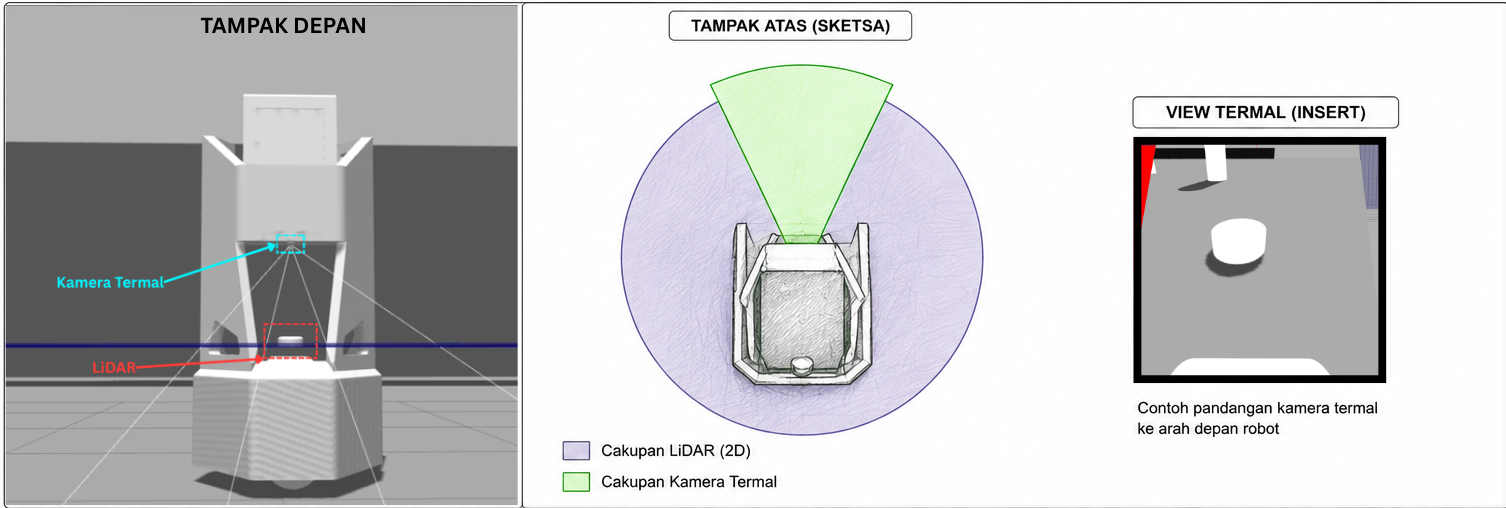
\includegraphics[width=0.85\textwidth]{gambar/3.4_lidar_thermal_fov.png}
\caption{Ilustrasi blind-spot vertikal pada sensor LiDAR dua dimensi.}
\label{fig:lidar_blindspot}
\end{figure}

\subsection{Deteksi Obstacle Terdekat}

Selain digunakan untuk membangun costmap, data LiDAR juga dimanfaatkan secara langsung oleh APFPlanner untuk menentukan jarak obstacle terdekat terhadap robot. Informasi ini diperlukan karena gaya tolak pada Artificial Potential Field bergantung pada jarak relatif antara robot dan obstacle.

Proses deteksi dilakukan dengan mencari nilai jarak minimum yang masih berada dalam rentang valid sensor. Misalkan himpunan data LiDAR dinyatakan sebagai

\begin{equation}
D = \{d_1,d_2,\dots,d_n\}
\end{equation}

maka jarak obstacle terdekat dapat diperoleh melalui

\begin{equation}
d_{obs} = \min(D)
\label{eq:min_obs_distance}
\end{equation}

dengan:

\begin{itemize}
\item $d_{obs}$ adalah jarak obstacle terdekat terhadap robot (m),
\item $D$ adalah himpunan data jarak valid dari LiDAR.
\end{itemize}

Nilai $d_{obs}$ selanjutnya digunakan sebagai salah satu variabel masukan pada pengendali fuzzy yang akan dibahas pada Subbab~\ref{sec:fuzzy_Aapf}.

\subsection{Estimasi Traversability Berbasis LiDAR}

Selain menghasilkan informasi jarak obstacle, data LiDAR juga digunakan untuk mengestimasi tingkat keterlaluan area di depan robot. Konsep traversability digunakan untuk mengg\-ambarkan seberapa aman suatu area untuk dilalui berdasarkan ruang bebas yang tersedia (\cite{Sevastopoulos2022}).

Pada penelitian ini, estimasi traversability LiDAR dilakukan dengan memanfaatkan informasi lebar koridor bebas di sekitar arah pergerakan robot. Semakin besar ruang bebas yang tersedia, semakin tinggi nilai traversability yang dihasilkan.

Lebar koridor bebas dinyatakan sebagai

\begin{equation}
w_{free}=x_{right}-x_{left}
\label{eq:free_width}
\end{equation}

dengan:

\begin{itemize}
\item $x_{right}$ adalah batas kanan area bebas,
\item $x_{left}$ adalah batas kiri area bebas.
\end{itemize}

Nilai traversability LiDAR kemudian dinormalisasi ke rentang $[0,1]$ sehingga dapat digunakan bersama traversability termal pada proses fusi sensor. Semakin mendekati 1, semakin besar area bebas yang tersedia untuk dilalui robot. Sebaliknya, nilai yang mendekati 0 menunjukkan bahwa area di depan robot semakin sempit atau dipenuhi obstacle.

Nilai traversability LiDAR yang dihasilkan pada tahap ini tidak digunakan secara langsung untuk navigasi, melainkan digabungkan dengan traversability termal pada proses fusi sensor yang dijelaskan pada Subbab~\ref{sec:fusi_traversability}.

